\newpage
\section{Visione generale della strategia di gestione della qualità}

	\subsection{Qualità di processo}
	Al fine di garantire la qualità del prodotto finale, è necessario garantire anche la qualità dei processi che porteranno al suo completamento. Lo standard ISO/IEC 15504, denominato SPICE, definisce come pianificare, eseguire, verificare e correggere ogni processo in modo costante. 
	Attenersi a questo standard permette di individuare e correggere ogni errore prima che esso si diffonda e provochi spreco di risorse. 
	
	Perché tutto questo sia possibile, bisogna utilizzare un metodo di controllo che siano ripetibili, oggettivi e comparabili. SPICE definisce 6 livelli di maturità del processo:
	
	\begin{itemize}
		\item 0 - Incomplete;
		\item 1 - Performed;
		\item 2 - Managed;
		\item 3 - Established;
		\item 4 - Predictable;
		\item 5 - Optimizing;
	\end{itemize}
	
	Al fine di applicare correttamente questo modello, è utile seguire il principio PDCA, il quale si compone di 4 fasi:
	
	\begin{itemize}
		\item \textbf{Plan: }definire dettagliatamente cosa deve essere realizzato rispetto agli obiettivi di miglioramento, e come questi controlli saranno effettuati;
		\item \textbf{Do: }fase di esecuzione delle attività pianificate;
		\item \textbf{Check: }vengono confrontati i dati in uscita dalla fase Do con quelli pianifcati nella fase Plan, per intervenire in tempo e migliorare i risultati;
		\item \textbf{Act: }fase in cui si mette in pratica il miglioramento continuo dei processi utilizzando i risultati della verifica per modificare gli aspetti critici dei processi in esame.
	\end{itemize}

	\begin{figure}[H]
		\centering
		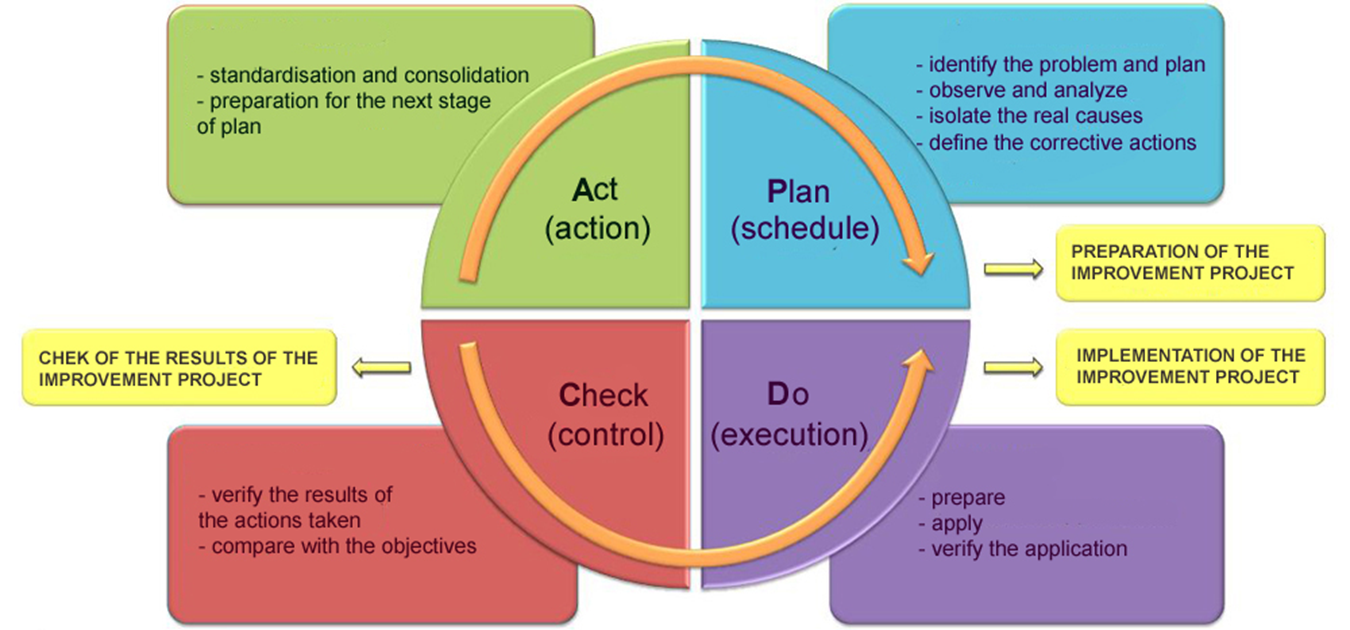
\includegraphics[scale=0.6]{includes/img/pdca.png}
		\caption{Fasi del principio PDCA.}
	\end{figure}
	
	\subsection{Qualità di prodotto}
	Al fine di avere un prodotto di qualità è necessario definire degli obiettivi di qualità e garantire che questi saranno raggiunti. 
	Lo standard ISO/IEC 9126 descrive obiettivi e metriche necessarie a valutarli.
	
	I criteri valutativi sono così suddivisi:
	
	\begin{itemize}
		\item \textbf{Qualità esterna: }le metriche esterne, specificate nella norma ISO/IEC 9126-2, valutano i comportamenti del prodotto sulla base di prove, dell'operatività e dell'osservazione durante la sua esecuzione, in funzione degli obiettivi stabiliti;
		\item \textbf{Qualità interna: }è specificata nella norma ISO/IEC 9126-3 e si applica al software non eseguibile
		durante la progettazione e la codifica dello stesso, le misure effettuate consentono di prevedere il livello di qualità esterna ed interna, in quanto gli attributi interni influenzano quelli esterni e di uso;
		\item \textbf{Qualità d'uso: }Rappresenta la qualità dal punto di vista dell'utente finale, viene raggiunto quando sono raggiunte la qualità esterna e quella interna, le metriche di valutazione sono fornite nella norma ISO/IEC 9126-4.
	\end{itemize}
	
	
	\subsection{Pianificazione strategica e temporale}
	Al fine di ridurre la propagazione di errori, l’attività di verifica di codice e documentazione dovrà essere sistematica. 
	Come procedura preliminare ad ogni attività, sarà necessario un studio preliminare volto ad evitare errori di natura tecnica o concettuale e conseguentemente alleggerire l’attività di verifica postuma.
	Si ha come obiettivo quello di rispettare e scadenze riportate nel \PdP.
	
	
	\subsection{Resposanbilità}
	Il \RdP ha il compito di:
	\begin{itemize}
		\item Accertarsi che attività e ruoli vengano rispettate, come definite nel \PdP;
		\item Accertarsi che le attività di verifica vengano eseguite sistematicamente, come descritto nelle \NdP;
		\item Approvarne un documento e sancirne la distribuzione.
	\end{itemize}

	I \Vers hanno il compito di:
	\begin{itemize}
		\item Effettuare l‘attività di verifica in modo sistematico utilizzando metodi e strumenti descritti nel \PdQ;
		\item Documentare e segnalare ogni errore riscontrato.
	\end{itemize}	
	
	
	\subsection{Risorse}
	Per la corretta riuscita del progetto sono necessarie risorse umane, software e hardware.
	
		\subsubsection{Risorse umane}
		\begin{itemize}
			\item \RdP;
			\item \Res;
			\item \Amm;
			\item \Ver;
			\item \Prog;
			\item \Ana.
		\end{itemize}
		
		\subsubsection{Risorse software}
		Sono necessari i software utili per
		\begin{itemize}
			\item la gestione di documentazione in \LaTeX;
			\item la creazione di diagrammi UML;
			\item lo sviluppo del codice nei linguaggi di programmazione scelti;
			\item l'automatizzazione e semplificazione delle attività di verifica;
			\item l'analisi statica del codice;
			\item la gestione dei test sul codice.
		\end{itemize}
		
		\subsubsection{Risorse hardware}
		\begin{itemize}
			\item personal computer dotati di tutti i software elencati nel \PdQ e nelle \NdP;
			\item luoghi dove effettuare le riunioni sia interne che esterne. In caso di riunioni esterne, potrebbe essere necessaria una connessione ad internet per un collegamento SKype con il cliente.
		\end{itemize}
		
						
	\subsection{Misure e metriche}
		Per conseguire dei risultati concreti, il processo di verifica deve fornire dei dati quantificabili per poter valutare se gli obiettivi sono stati raggiunti o meno. Queste è possibile tramite l’utilizzo di metriche e misure. Considerata la quasi nulla esperienza del gruppo, questi valori potrebbero essere inizialmente poco accurati, ma utilizzando il modello incrementale visto nel Piano di Progetto si potrà migliorarne la precisione.
		Per ogni metrica sono indicati due range:
		\begin{itemize}
			\item \textbf{Range-accettazione: }rappresenta i valori minimi da raggiungere per il conseguimento degli obiettivi di qualità;
			\item \textbf{Range-ottimale: }rappresenta i valori entro cui dovrebbe collocarsi la misurazione. Non sono vincolanti ma nel caso in cui non si raggiungessero questi valori, sarà necessaria una verifica più accurata e una ulteriore discussione, nella riunione successiva, delle cause di questo scostamento.
		\end{itemize}
	
		\subsubsection{Metriche per i documenti}
		
		\subsubsection{Indice Gulpease }
		L'Indice Gulpease è un indice di leggibilità di un testo tarato sulla lingua italiana. Rispetto ad altri ha il vantaggio di utilizzare la lunghezza delle parole in lettere anziché in sillabe, semplificandone il calcolo automatico.
		L'indice di Gulpease considera due variabili linguistiche: la lunghezza della parola e la lunghezza della frase rispetto al numero delle lettere.
		La formula per il suo calcolo è la seguente:
		
		\[ 80+\frac{300*(numero delle frasi)-10*(numero delle lettere)}{numero delle parole} \]
		
		
		I risultati sono compresi tra 0 e 100, dove il valore "100" indica la leggibilità più alta e "0" la leggibilità più bassa. In generale risulta che testi con un indice:
		\begin{itemize}
			\item inferiore a 80 sono difficili da leggere per chi ha la licenza elementare;
			\item inferiore a 60 sono difficili da leggere per chi ha la licenza media;
			\item inferiore a 40 sono difficili da leggere per chi ha un diploma superiore.
		\end{itemize}
	
		I parametri presi in considerazione saranno:
	
		\begin{itemize}
			\item \textbf{Range-accettazione: }[35/100];
			\item \textbf{Range-ottimale: }[45/100].
		\end{itemize}
	
		\subsubsection{Metriche per i processi}
		Le metriche scelte prendono in considerazione tempi e costi, in modo da poter controllare efficacemente i processi e riuscire ad attenersi a quanto deciso nel Piano di Progetto. 
		Per queste metriche non viene non vengono forniti Range-accetazione e Range-ottimale poiché bisognerà consultare il Piano di Progetto per fare le dovute considerazioni.
		
		\begin{itemize}
			\item \textbf{PPC (Partial Planned Cost): }indica il costo pianificato per lo svolgimento di un sottoinsieme di attività. Si misura in euro e in ore;
			\item \textbf{PV (Planned Value): }indica il valore che si prevede ottenere dal completamento delle attività pianificate. Per questo progetto tale valore corrisponde alla spesa richiesta per il completamento delle attività. Si misura in euro e in ore;
			\item \textbf{EV (Earned Value): }indica il valore ottenuto tramite le attività completate alla data corrente. Per questo progetto tale valore corrisponde alla spesa richiesta per il completamento delle attività. Si misura in euro e in ore;
			\item \textbf{AC (Actual Cost): }indica il costo effettivamente sostenuto alla data corrente. Si misura in euro e in ore. Aiuta a calcolare altre metriche;
			\item \textbf{BAC (Budget at Completion): }costo previsto per portare a termine il progetto. Si misura in euro e in ore. Mantiene traccia della spesa totale preventivata all'inizio del progetto;
			\item \textbf{ETC (Estimate to Complete): }indica i costi pianificati per portare a termine le attività di progetto rimanenti alla data corrente. Corrisponde al PV riesaminato allo stato corrente del progetto ma senza tenere conto delle attività completate. Si misura in euro e in ore;
			\item \textbf{EAC (Estimated at Completion): }revisione del costo stimato per la realizzazione del progetto, ossia il BAC rivisto allo stato corrente del progetto. Si misura in euro e in ore e si ottiene dalla formula: EAC = AC + ETC;
			\item \textbf{SV (Schedule Variance): }è un indicatore di efficacia, mostra se si è o meno in linea con la pianificazione temporale rispetto alle attività nella baseline. Una schedule variance positiva indica che il gruppo è in anticipo rispetto al Piano di progetto, che è in ritardo altrimenti. Si ottiene dalla formula: SV = EV - PV;
			\item \textbf{BV (Budget Variance): }indica se la spesa sostenuta alla data corrente è superiore o inferiore a quella preventivata. Una budget variance positiva indica che si è speso meno di quanto inizialmente previsto, viceversa altrimenti. Si ottiene dalla formula: BV = PV - AC.
			
		\end{itemize}
		
		
		\subsubsection{Metriche per il codice}
		Le metriche per il software ora descritte non sono definitive, ma saranno affinate successivamente.
		
		\begin{itemize}
			\item \textbf{Attributi per classe: }in grande numero di attributi interni ad una classe mostra probabilmente la necessità di suddividere la classe in più classi relazionate tra loro.
			
			\begin{itemize}
				\item \textbf{Range-accettazione: }[0/18];
				\item \textbf{Range-ottimale: }[2/9].
			\end{itemize}
		
			\item \textbf{Numero livelli annidamento: }mostra il livello di annidamento dei metodi. Un numero alto implica una bassa astrazione del codice ed un' elevata complessità.
			
			\begin{itemize}
				\item \textbf{Range-accettazione: }[1/8];
				\item \textbf{Range-ottimale: }[1/4].
			\end{itemize}
			
			\item \textbf{Numero parametri per metodo: }un valore elevato indica che probabilmente il metodo ha un sovraccarico di funzionalità.
			
			\begin{itemize}
				\item \textbf{Range-accettazione: }[0/8];
				\item \textbf{Range-ottimale: }[0/5].
			\end{itemize}
			
			\item \textbf{Accoppiamento afferente: }indica il numero di classi esterne ad un package che dipendono da esso. Un grande valore indica una forte dipendenza del software per il package in questione, un valore basso invece indica una bassa utilità del package per il resto del software.
			
			\begin{itemize}
				\item \textbf{Range-accettazione: }non ancora definito;
				\item \textbf{Range-ottimale: }non ancora definito.
			\end{itemize}
			
			\item \textbf{Accoppiamento efferente: }il numero di classi di un package che dipendono da package esterni. Un valore basso indica che il package ha numerose funzionalità indipendenti dal resto del software.
			
			\begin{itemize}
				\item \textbf{Range-accettazione: }non ancora definito;
				\item \textbf{Range-ottimale: }non ancora definito.
			\end{itemize}
			
			\item \textbf{Source Line Of Code (SLOC): }il numero di istruzioni presenti nel codice. Questa metrica fornisce una stima della complessità del programma. È utile anche per dare una stima di quanto il codice incrementerà nel tempo, semplificando così la pianificazione.
			
			\begin{itemize}
				\item \textbf{Range-accettazione: }[0/18];
				\item \textbf{Range-ottimale: }[2/9].
			\end{itemize}
			
			\item \textbf{Complessità Ciclomatica: }una metrica sviluppata da Thomas J. McCabe che consente di stimare la complessità di un programma misurando il numero di cammini linearmente indipendenti attraverso il grafo di controllo di flusso.
			
			\begin{itemize}
				\item \textbf{Range-accettazione: }non ancora definito;
				\item \textbf{Range-ottimale: }non ancora definito.
			\end{itemize}
			
			
		
		\end{itemize}
		
		
	\subsection{Analisi}
	
		\subsubsection{Analisi statica}
		L'analisi statica non necessità dell'esecuzione del codice oggetto ed è per cui applicabile sin da subito su codice e documenti prodotti. Essa ha lo scopo di trovare anomalie e può essere eseguita nei due modi seguenti.
		
		\subsubsection{Walkthrough}
		Questa tecnica consistente nella ricerca a largo spettro di qualsiasi tipo di errore, nel modo più generico possibile. 
		Questa tecnica è utilizzata nelle prime fasi di verifica. Durante ogni fase di verifica verrà stilata una lista degli errori più frequenti, in modo da facilitare l’individuazione delle anomalie nelle fasi successive. 
		Ne momento in cui si avrà a disposizione una lista sufficientemente dettagliata, si potrà passare al metodo Inspection.
		
		
		\subsubsection{Inspection}
		Questo metodo si basa sulla lista prodotta precedentemente con il metodo Walkthrough. In questo modo si andrà a cercare in modo mirato gli errori già individuati in passato, prestando comunque attenzione a nuovi possibili errori, che andranno poi ad arricchire la lista
		
		
		\subsubsection{Analisi dinamica}
		Da definire
		
		
	